\documentclass[a4paper,11pt]{article}

\usepackage[utf8]{inputenc}
\usepackage[top=2cm, left = 2cm , right=2cm , bottom=2cm]{geometry}
\usepackage{amsmath}
\usepackage{graphicx}
\usepackage{float}
\usepackage{listings}
\usepackage[brazil]{babel}

\usepackage{color}

\definecolor{mygreen}{rgb}{0,0.6,0}
\definecolor{mygray}{rgb}{0.5,0.5,0.5}
\definecolor{mymauve}{rgb}{0.58,0,0.82}

\lstset{
  backgroundcolor=\color{white},   % choose the background color; you must add
                                   % \usepackage{color} or \usepackage{xcolor};
                                   % should come as last argument
  basicstyle=\footnotesize,        % the size of the fonts
  breakatwhitespace=false,         % sets if automatic breaks should only happen
                                   % at whitespace
  breaklines=true,                 % sets automatic line breaking
  captionpos=b,                    % sets the caption-position to bottom
  commentstyle=\color{mygreen},    % comment style
  escapeinside={\%*}{*)},          % if you want to add LaTeX within your code
  extendedchars=true,              % lets you use non-ASCII characters; for
                                   % 8-bits encodings only, does not work with
                                   % UTF-8
  frame=single,	                 % adds a frame around the code
  keepspaces=true,                 % keeps spaces in text, useful for keeping
                                   % indentation of code (possibly needs
                                   % columns=flexible)
  keywordstyle=\color{blue},       % keyword style
  language=Matlab,                 % the language of the code
  numbers=left,                    % where to put the line-numbers; possible
                                   % values are (none, left, right)
  numbersep=5pt,                   % how far the line-numbers are from the code
  numberstyle=\tiny\color{mygray}, % the style that is used for the line-numbers
  rulecolor=\color{black},         % if not set, the frame-color may be changed
                                   % on line-breaks within not-black text
                                   % (e.g. comments (green here))
  showspaces=false,                % show spaces everywhere adding particular
                                   % underscores; it overrides
                                   % 'showstringspaces'
  showstringspaces=false,          % underline spaces within strings only
  showtabs=false,                  % show tabs within strings adding particular
                                   % underscores
  stepnumber=2,                    % the step between two line-numbers. If it's
                                   % 1, each line will be numbered
  stringstyle=\color{mymauve},     % string literal style
  tabsize=2,                       % sets default tabsize to 2 spaces
  title=\lstname                   % show the filename of files included with
                                   % \lstinputlisting; also try caption instead
                                   % of title
}

\pagestyle{plain}

\begin{document}

\begin{center}
\textbf{Experiência 1}\\ \hspace{5pt}Prof. Marconi Kolm Madrid\\EA772 - 2017/2
\end{center}

\begin{center}
Danilo Pereira Titato - RA 122541\\
Giovani Granzotto Oliani - RA 146253\\
Pedro Gabriel Calixto Mendonça - RA 118363\\
\end{center}

1. Problema do servo

\begin{gather*}
    G^\prime_{p_s} := \frac{X_1 \left( s \right)}{F_a \left( s \right)} \\
    X_{1} \left( s \right) = \frac{1}{m_1s^2 + c_1s + k_1} \cdot k_{hw} \cdot
        \left( F_a \left( s \right) - k_vs \cdot X_1 \left( s \right) \right) \\
    X_{1} \left( s \right) \cdot \left( 1 + \frac{k_{hw} \cdot k_v \cdot s}
        {m_1s^2 + c_1s + k_1} \right) = F_a\left( s \right) \cdot
        \frac{k_{hw}}{m_1s^2 + c_1s + k_1} \\
    X_{1} \left( s \right) \cdot \left[ m_1s^2 + \left( c_1 k_{hw} k_v \right) s
        + k_1 \right] = F_a\left( s \right) \cdot k_{hw}
\end{gather*}
\begin{equation}
    \label{eq:Gps}
    G^\prime_{p_s} = \frac{X_{1}\left( s \right)}{F_a\left( s \right)} =
         \frac{k_{hw}}{m_1s^2 + \left( c_1 k_{hw} k_v \right) s + k_1},
         C.Q.D.
\end{equation}

2. Problema da regulação

\begin{gather*}
    G^\prime_{p_r} := \frac{X_1 \left( s \right)}{F_p \left( s \right)} \\
    X_{1} \left( s \right) = \frac{1}{m_1s^2 + c_1s + k_1} \cdot \left(
        F_p\left( s \right) - k_{hw} \cdot k_vs \cdot X_1 \left( s \right)
        \right) \\
    X_{1} \left( s \right) \cdot \left( 1 + \frac{k_{hw} \cdot k_v \cdot s}
        {m_1s^2 + c_1s + k_1} \right) = F_p \left( s \right) \cdot
        \frac{1}{m_1s^2 + c_1s + k_1} \\
    X_{1} \left( s \right) \cdot \left[ m_1s^2 + \left( c_1 k_{hw} k_v \right) s
        + k_1 \right] = F_p\left( s \right)
\end{gather*}
\begin{equation}
    \label{eq:Gpr}
    G^\prime_{p_r} = \frac{X_{1}\left( s \right)}{F_p\left( s \right)} =
         \frac{1}{m_1s^2 + \left( c_1 k_{hw} k_v \right) s + k_1}, C.Q.D.
\end{equation}

Substituindo $k_1$ por $k_1^\ast$, como deve ser feito para a simulação de
perturbação:

\begin{gather*}
    G^\prime_{p_r^\ast} =
         \frac{1}{m_1s^2 + \left( c_1 k_{hw} k_v \right) s + k_1^\ast} =
         \frac{1}{m_1s^2 + \left( c_1 k_{hw} k_v \right) s +
         \left( k_1 + \Delta k_1 \right)}.
\end{gather*}

\newpage

3. (a) Os valores de ganho de baixa frequência calculados para o $G^\prime_{p_s}$ são:

\begin{gather*}
    G^\prime_{p_s} \left( 0 \right) = \frac{14372}{2.778 \cdot s^2 + 76.6 \cdot
      s + 338.6} \approx 43.5086 \\ \\
    G^\prime_{p_s^\ast} \left( 0 \right) = \frac{14372}{2.778 \cdot s^2 + 76.6
      \cdot s + 700} \approx 21.0457
\end{gather*}

O \textit{script} desenvolvido em Matlab para gerar a função de transferência e
obter os valores de ganho de baixa frequência foi:

\begin{lstlisting}
% parametros iniciais
s = tf('s');

mc1 = 0.778;
mw1 = 4*0.500;
m1 = mc1 + mw1;

c1 = 2.94;
kv = 0.005;
khw = 14732;

k1 = 338.6;
deltak1 = 361.4;

% Gps eh a funcao de transferencia da "planta compensada" para o problema servo
% GpsDelta eh Gps*, a funcao de transferencia para o valor perturbado
Gps = khw / (m1*s^2 + (c1+khw*kv)*s + k1);
GpsDelta = khw / (m1*s^2 + (c1+khw*kv)*s + (k1 + deltak1));

display(tf(Gps));
display(tf(GpsDelta));

% ganhos de baixa frequencia
Gps0 = dcgain(Gps);
Gps0Delta = dcgain(GpsDelta);

display(Gps0);
display(Gps0Delta);
\end{lstlisting}

Os resultados obtidos no Matlab são:

\begin{lstlisting}
ans =
            14732
  --------------------------
  2.778 s^2 + 76.6 s + 338.6
 
Continuous-time transfer function.

ans =
           14732
  ------------------------
  2.778 s^2 + 76.6 s + 700
 
Continuous-time transfer function.

Gps0 =
   43.5086

Gps0Delta =
   21.0457
\end{lstlisting}

Como pode-se ver, os resultados são exatamente iguais aos calculados. \\

(b) Os valores de ganho de baixa frequência calculados para o $G^\prime_{p_r}$
são:

\begin{gather*}
    G^\prime_{p_r} \left( 0 \right) = \frac{1}{2.778 \cdot s^2 + 76.6 \cdot s +
        338.6} \approx 0.00295334 \\ \\
    G^\prime_{p_r^\ast} \left( 0 \right) = \frac{1}{2.778 \cdot s^2 + 76.6 \cdot
      s + 700} \approx 0.00142857
\end{gather*}

O \textit{script} desenvolvido em Matlab para obter os valores de ganho de baixa
frequência, considerando os já implementados parâmetros inicias, foi:

\begin{lstlisting}
% funcoes de transferencia
Gpr = 1 / (m1*s^2 + (c1+khw*kv)*s + k1);
GprDelta = 1 / (m1*s^2 + (c1+khw*kv)*s + (k1 + deltak1));

display(tf(Gpr));
display(tf(GprDelta));

% ganhos de baixa frequencia
Gpr0 = dcgain(Gpr);
Gpr0Delta = dcgain(GprDelta);

display(Gpr0);
display(Gpr0Delta);
\end{lstlisting}

Os resultados obtidos no Matlab são:

\begin{lstlisting}
ans =
              1
  --------------------------
  2.778 s^2 + 76.6 s + 338.6

Continuous-time transfer function.

ans =
             1
  ------------------------
  2.778 s^2 + 76.6 s + 700
 
Continuous-time transfer function.

Gpr0 =
    0.0030

Gpr0Delta =
    0.0014
\end{lstlisting}

Como pode-se ver, os resultados são exatamente iguais aos calculados. \\

(c)

\begin{lstlisting}
display(Gps0Delta - Gps0);
display(Gpr0Delta - Gpr0);
\end{lstlisting}

\begin{lstlisting}
  -22.4629
   -0.0015
\end{lstlisting}

(d)

\begin{lstlisting}
% parametros iniciais
Gpf = 1;
kp = 0.12;

% funcoes de transferencia
Ga = Gpf * Gps;
GaDelta = Gpf * GpsDelta;

Gf = Gpf * feedback(Gps * kp, 1);
GfDelta = Gpf * feedback(GpsDelta * kp, 1);

display(tf(Ga));
display(tf(GaDelta));
display(tf(Gf));
display(tf(GfDelta));
\end{lstlisting}

\begin{lstlisting}
ans =
            14732
  --------------------------
  2.778 s^2 + 76.6 s + 338.6
 
Continuous-time transfer function.


ans =
           14732
  ------------------------
  2.778 s^2 + 76.6 s + 700
 
Continuous-time transfer function.

ans =
            1768
  -------------------------
  2.778 s^2 + 76.6 s + 2106
 
Continuous-time transfer function.


ans =
            1768
  -------------------------
  2.778 s^2 + 76.6 s + 2468
 
Continuous-time transfer function.
\end{lstlisting}

(e)

\begin{gather*}
    G\left(s\right) = \frac{X_1\left(s\right)}{X_{1r}\left(s\right)} \implies
         X_1\left(s\right) = G\left(s\right) \cdot X_{1r}\left(s\right)
\end{gather*}
\begin{align*}
\label{eq:1}
    e_r = \lim_{s\to0} sE\left(s\right) &= \lim_{s\to0} s \cdot \left(X_{1r}
        \left(s\right) - X_1\left(s\right)\right) \\
    &= \lim_{s\to0} s \cdot \left(X_{1r}\left(s\right) - G\left(s\right) \cdot
        X_{1r}\left(s\right)\right) \\
    &= \lim_{s\to0} s \cdot X_{1r}\left(s\right) \cdot
        \left(1 - G\left(s\right)\right)
\end{align*}

Dado que a entrada $x_{1r}$ é o degrau unitário; $X_{1r}$, que é a sua
transformada, é igual a $1/s$. Logo:

\begin{gather*}
    e_r = \lim_{s\to0} s \cdot \frac{1}{s} \cdot
        \left(1 - G\left(s\right)\right)
\end{gather*}
\begin{equation} \label{eq:erro-de-reg}
    e_r = \lim_{s\to0} 1 - G\left(s\right)
\end{equation}

O \textit{script} para obter os valores de erro de regime dos sistemas em malha
aberta e em malha fechada foi, então:

\begin{lstlisting}
% calculo dos erros de regime
eRegA = dcgain(1 - Ga);
eRegADelta = dcgain(1 - GaDelta);

eRegF = dcgain(1 - Gf);
eRegFDelta = dcgain(1 - Gfdelta);

display(eRegA);
display(eRegF);
display(eRegADelta);
display(eRegFDelta);
\end{lstlisting}

\begin{lstlisting}
eRegA =
  -42.5086

eRegF =
    0.1607

eRegADelta =
  -20.0457

eRegFDelta =
    0.2836
\end{lstlisting}

Como podemos ver, para $k_1$ e $k_1^\ast$, os valores de erro de regime são
bem menores em malha fechada do que em malha aberta, respectivamente.
Isso se dá por conta da regulação obtida pela realimentação do sinal de saída
$x_1$. \\

(f) O \textit{script} desenvolvido em Matlab para gerar as respostas ao degrau
dos sistemas (considerando $k_1$ e $k_{1r}$ em malha aberta e em malha fechada
foi:

\begin{lstlisting}
% respostas ao degrau
[stepGa, tA] = step(Ga, 1.2);
[stepGaDelta, tADelta] = step(GaDelta, 1.2);
[stepGf, tF] = step(Gf, 1.2);
[stepGfDelta, tFDelta] = step(GfDelta, 1.2);

% funcoes degrau para malha aberta e fechada
degrauA = ones(length(stepGa), 1);
degrauF = ones(length(stepGf), 1);

% graficando malha aberta para k1 e k1*
figure, plot(tA, degrauA, tA, stepGa, tADelta, stepGaDelta);
title('Malha aberta');
legend('degrau', 'k1', 'k1*', 'Location', 'northwest');

% graficando malha fechada para k1 e k1*
figure, plot(tF, degrauF, tF, stepGf, tFDelta, stepGfDelta);
title('Malha fechada');
legend('degrau', 'k1', 'k1*', 'Location', 'southeast');
\end{lstlisting}

Os gráficos gerados são:

\begin{figure}[H]
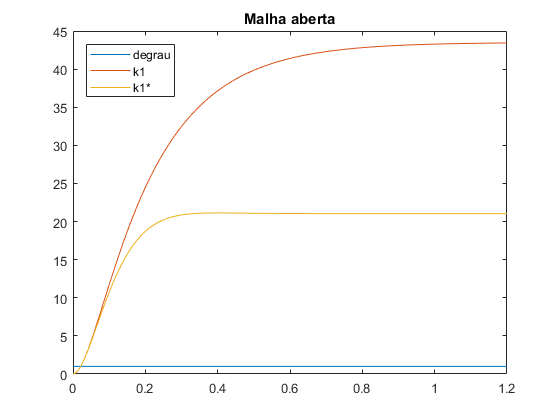
\includegraphics{exp01e03f-aberta}
\centering
\end{figure}

\begin{figure}[H]
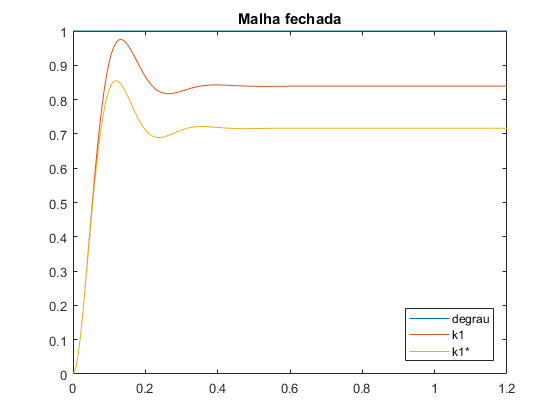
\includegraphics{exp01e03f-fechada}
\centering
\end{figure}

4. Para que o erro de regime de malha aberta seja mínimo (nulo), usando a
equações~\ref{eq:Gps} e~\ref{eq:erro-de-reg}:

\begin{gather*}
    \lim_{s\to0} 1 - G_a\left(s\right) = 0 \implies \\
    \lim_{s\to0} 1 - G_{pf}\left(s\right) \cdot
        G^\prime_{p_s}\left(s\right) =
        \lim_{s\to0} 1 - k_{pf} \cdot
        \frac{k_{hw}}{m_1s^2 + \left( c_1 k_{hw} k_v \right) s + k_1} =
        1 - k_{pf} \cdot \frac{k_{hw}}{k_1} = 0 \implies \\
    k_{pf} = \frac{k_1}{k_{hw}}
\end{gather*}

\end{document}